%% GA-HBF for Near-Field STAR-RIS Networks
%% Restyled to CA-SUS visual language (ATC conflict-aware deck)
%%   pdflatex GA_HBF_STAR_RIS_presentation.tex
\documentclass[aspectratio=169,11pt]{beamer}

\usetheme{default}
\usecolortheme{default}
\setbeamertemplate{navigation symbols}{}

\definecolor{navyblue}{RGB}{0,51,102}
\definecolor{darkblue}{RGB}{0,51,102}
\definecolor{softblue}{RGB}{232,240,248}
\definecolor{softgreen}{RGB}{226,242,226}
\definecolor{notegreen}{RGB}{34,102,68}
\definecolor{titlebar}{RGB}{0,40,85}

\setbeamercolor{structure}{fg=navyblue}
\setbeamercolor{frametitle}{bg=navyblue,fg=white}
\setbeamercolor{title}{fg=black}
\setbeamercolor{block title}{bg=titlebar,fg=white}
\setbeamercolor{block body}{bg=softblue,fg=black}
\setbeamercolor{item}{fg=navyblue}
\setbeamerfont{frametitle}{size=\large}
\setbeamertemplate{itemize item}[circle]
\setbeamertemplate{bibliography item}[text]
\setbeamertemplate{caption}{\insertcaption}
\setbeamertemplate{footline}{}

\usepackage[T1]{fontenc}
\usepackage[utf8]{inputenc}
\usepackage{amsmath,amssymb,bm}
\usepackage{graphicx}
\usepackage{tikz}
\usetikzlibrary{arrows.meta,positioning,fit,calc}

\graphicspath{{presentation_figs/}}

\newcommand{\confbanner}{ATC 2026, 15--17 October 2026, Quy Nhon, Vietnam}
\newcommand{\confshort}{ATC 2026}
\newcommand{\conffull}{2026 International Conference on Advanced Technologies for Communications}

% Paper notation
\newcommand{\vT}{v_T}
\newcommand{\vR}{v_R}

\newcommand{\ctxbox}[2]{%
  \noindent
  \begin{tikzpicture}
    \node[draw=navyblue, rounded corners, fill=softblue,
          inner sep=8pt, text width=0.92\textwidth, align=left] {
      {\normalsize\textbf{#1}}~{\normalsize #2}};
  \end{tikzpicture}\\[0.55em]}


\begin{document}

%======================================================================
% TITLE --- CA-SUS title chrome
%======================================================================
\begin{frame}[plain]
\begin{tikzpicture}[remember picture, overlay]
\fill[darkblue] (current page.north west) rectangle ([yshift=-3.2cm]current page.north east);
\node[white, font=\small\bfseries] at ([yshift=-0.45cm]current page.north)
    {\confbanner};
\node[white, font=\Large\bfseries] at ([yshift=-1.5cm]current page.north) {\confshort};
\node[white, font=\normalsize] at ([yshift=-2.5cm]current page.north)
    {\conffull};
\node[black, font=\large\bfseries, text width=0.94\textwidth, align=center]
    at ([yshift=-4.8cm]current page.north)
    {Low-Complexity Geometry-Aware Hybrid Beamforming\\
     for Near-Field STAR-RIS Networks};
\node[black, font=\small, text width=0.94\textwidth, align=center]
    at ([yshift=-6.5cm]current page.north)
    {Nam Van Dinh, Nguyen Tien Hoa, Ngo Hoang Tu,\\
     Vo Nguyen Quoc Bao, Hai Minh Truong, Thuan Van Le};
\node[black, font=\small\bfseries] at ([yshift=-7.5cm]current page.north)
    {Presented By: Ngo Hoang Tu};
\end{tikzpicture}
\end{frame}

%======================================================================
% 1. CONTEXT
%======================================================================
\begin{frame}{1. Context \& Motivation}
  \ctxbox{STAR-RIS:}{A simultaneously transmitting and reflecting surface that covers both sides of space.
    In energy-splitting mode each element sends part of the energy through and reflects the rest.
    Users only receive; the T-side or R-side is decided by location.}
  \ctxbox{Hybrid beamforming:}{The base station uses a limited number of RF chains.
    Analog phase shifters plus a small digital precoder keep hardware cost low,
    so only a few users can be scheduled in each slot.}
  \ctxbox{Constraint:}{One common profile per side couples user scheduling, energy splitting, and beamforming.
    Iterative joint optimization grows fast with the surface size, and gain-only scheduling keeps favoring
    a few users whose effective channels can still be highly correlated.}
\end{frame}

%======================================================================
% 2. OVERALL ARCHITECTURE
%======================================================================
\begin{frame}{2. Overall Architecture}
  \centering
  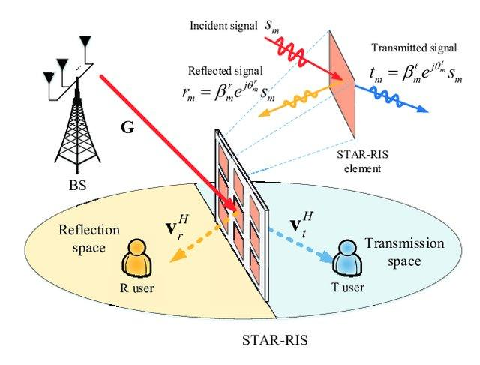
\includegraphics[width=0.78\textwidth,height=0.48\textheight,keepaspectratio]{ref_star_ris.pdf}\\[0.15em]
  {\scriptsize STAR-RIS architecture}\\[0.45em]
  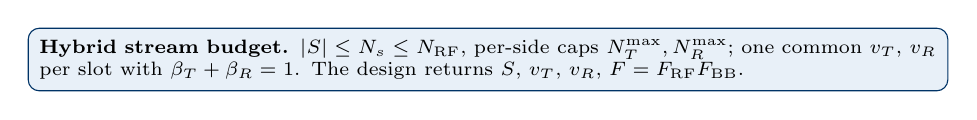
\begin{tikzpicture}
    \node[draw=navyblue, rounded corners, fill=softblue,
          align=left, inner sep=4pt, text width=0.94\textwidth, font=\scriptsize] {
      \textbf{Hybrid stream budget.}
      $|S|\le N_s\le N_{\mathrm{RF}}$, per-side caps $N_T^{\max}, N_R^{\max}$;
      one common $v_T$, $v_R$ per slot with $\beta_T+\beta_R=1$. The design returns $S$, $v_T$, $v_R$, $F=F_{\mathrm{RF}}F_{\mathrm{BB}}$.};
  \end{tikzpicture}\\[0.35em]
  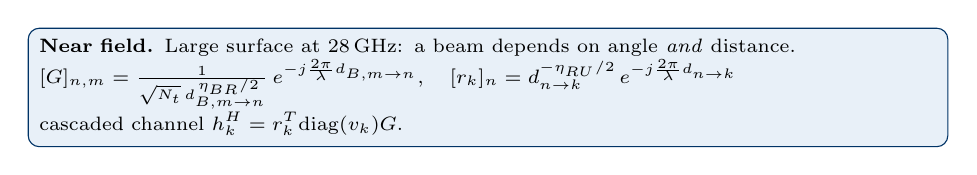
\begin{tikzpicture}
    \node[draw=navyblue, rounded corners, fill=softblue,
          align=left, inner sep=4pt, text width=0.94\textwidth, font=\scriptsize] {
      \textbf{Near field.}
      Large surface at 28\,GHz: a beam depends on angle \emph{and} distance.\\
      $[G]_{n,m}=\frac{1}{\sqrt{N_t}\,d_{B,m\to n}^{\,\eta_{BR}/2}}\,e^{-j\frac{2\pi}{\lambda}d_{B,m\to n}},\quad
      [r_k]_n=d_{n\to k}^{-\eta_{RU}/2}\,e^{-j\frac{2\pi}{\lambda}d_{n\to k}}$\\
      cascaded channel $h_k^H=r_k^T\mathrm{diag}(v_k)G$.};
  \end{tikzpicture}
\end{frame}

%======================================================================
% 3. THREE INGREDIENTS IN PSI(S)
%======================================================================
\begin{frame}{3. Three Ingredients Aligned in $\Psi(S)$}
  \vspace{0.05cm}
  \begin{center}
  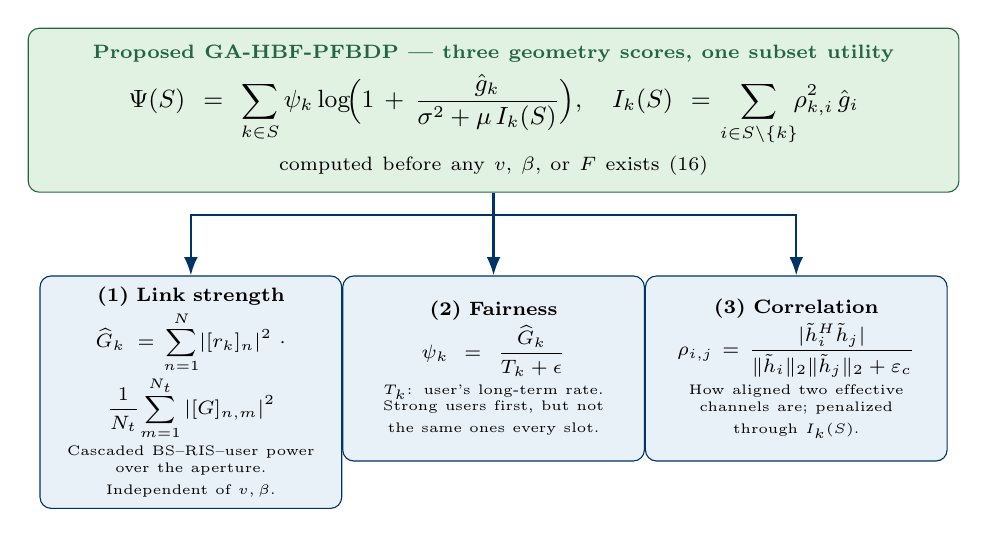
\begin{tikzpicture}[
      arr/.style={-{Latex}, thick, navyblue},
      card/.style={draw=navyblue, rounded corners, fill=softblue,
                   align=center, inner sep=4pt, font=\scriptsize,
                   text width=3.55cm, minimum height=2.35cm},
      etabox/.style={draw=notegreen, rounded corners, fill=softgreen,
                    align=center, inner sep=6pt}
    ]
    \node[etabox, text width=0.94\textwidth] (psi) {%
      {\scriptsize\color{notegreen}\textbf{Proposed GA-HBF-PFBDP --- three geometry scores, one subset utility}}\\[0.35em]
      {\small $\displaystyle\Psi(S)=\sum_{k\in S}\psi_k\log\!\Bigl(1+\frac{\hat g_k}{\sigma^2+\mu\,I_k(S)}\Bigr),
      \quad I_k(S)=\!\!\sum_{i\in S\setminus\{k\}}\!\!\rho_{k,i}^2\,\hat g_i$}\\[0.3em]
      {\scriptsize computed before any $v$, $\beta$, or $F$ exists (16)}};
    \node[card, below=1.05cm of psi.south west, xshift=0.15cm, anchor=north west] (f1) {%
      \textbf{(1) Link strength}\\[0.1em]
      $\displaystyle\widehat{G}_k=\!\sum_{n=1}^{N}\!|[r_k]_n|^2\cdot\frac1{N_t}\!\sum_{m=1}^{N_t}|[G]_{n,m}|^2$\\[0.15em]
      {\tiny Cascaded BS--RIS--user power\\over the aperture.\\Independent of $v,\beta$.}};
    \node[card, below=1.05cm of psi.south, anchor=north] (f2) {%
      \textbf{(2) Fairness}\\[0.1em]
      $\displaystyle\psi_k=\frac{\widehat{G}_k}{T_k+\epsilon}$\\[0.25em]
      {\tiny $T_k$: user's long-term rate.\\Strong users first, but not\\the same ones every slot.}};
    \node[card, below=1.05cm of psi.south east, xshift=-0.15cm, anchor=north east] (f3) {%
      \textbf{(3) Correlation}\\[0.1em]
      $\displaystyle\rho_{i,j}=\frac{|\tilde h_i^H\tilde h_j|}{\|\tilde h_i\|_2\|\tilde h_j\|_2+\varepsilon_c}$\\[0.2em]
      {\tiny How aligned two effective\\channels are; penalized\\through $I_k(S)$.}};
    \draw[arr] (psi.south) -- ++(0,-0.28) -| (f1.north);
    \draw[arr] (psi.south) -- (f2.north);
    \draw[arr] (psi.south) -- ++(0,-0.28) -| (f3.north);
  \end{tikzpicture}
  \end{center}
\end{frame}

%======================================================================
% 4. HOW S IS CHOSEN + HOW ONE SURFACE SERVES BOTH SIDES
%======================================================================
\begin{frame}{4. Who Is Served ($S$) and How One Surface Serves Both Sides}
  \vspace{-0.15cm}
  \begin{center}
  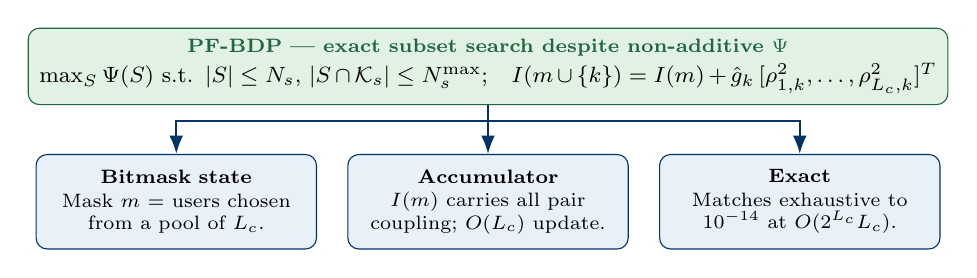
\begin{tikzpicture}[
      arr/.style={-{Latex}, thick, navyblue},
      eqbox/.style={draw=notegreen, rounded corners, fill=softgreen,
                    align=center, inner sep=4pt, font=\footnotesize},
      card/.style={draw=navyblue, rounded corners, fill=softblue,
                   align=center, inner sep=3pt, font=\scriptsize,
                   text width=3.35cm, minimum height=1.2cm}
    ]
    \node[eqbox, text width=0.94\textwidth] (eq) {%
      {\scriptsize\color{notegreen}\textbf{PF-BDP --- exact subset search despite non-additive $\Psi$}}\\[0.15em]
      $\max_S\Psi(S)$ s.t. $|S|\le N_s$, $|S\cap\mathcal{K}_s|\le N_s^{\max}$;\quad
      $I(m\cup\{k\})=I(m)+\hat g_k\,[\rho_{1,k}^2,\dots,\rho_{L_c,k}^2]^T$};
    \node[card, below=0.62cm of eq.south west, xshift=0.1cm, anchor=north west] (g1) {%
      \textbf{Bitmask state}\\[0.08em]
      Mask $m$ = users chosen\\
      from a pool of $L_c$.};
    \node[card, below=0.62cm of eq.south, anchor=north] (g2) {%
      \textbf{Accumulator}\\[0.08em]
      $I(m)$ carries all pair\\
      coupling; $O(L_c)$ update.};
    \node[card, below=0.62cm of eq.south east, xshift=-0.1cm, anchor=north east] (g3) {%
      \textbf{Exact}\\[0.08em]
      Matches exhaustive to\\
      $10^{-14}$ at $O(2^{L_c}L_c)$.};
    \draw[arr] (eq.south) -- ++(0,-0.2) -| (g1.north);
    \draw[arr] (eq.south) -- (g2.north);
    \draw[arr] (eq.south) -- ++(0,-0.2) -| (g3.north);
  \end{tikzpicture}\\[0.8em]
  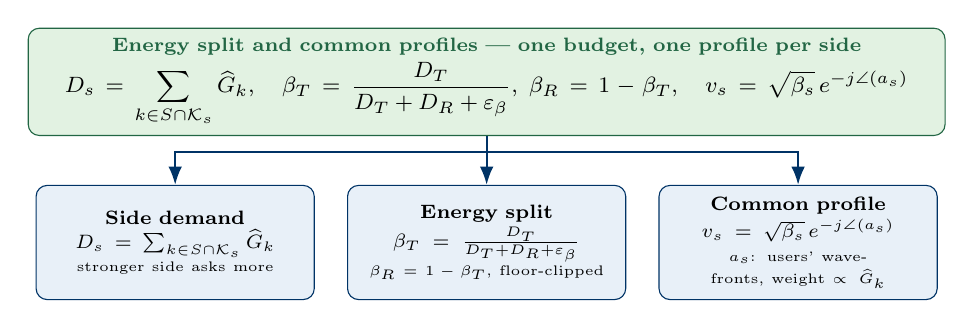
\begin{tikzpicture}[
      arr/.style={-{Latex}, thick, navyblue},
      eqbox/.style={draw=notegreen, rounded corners, fill=softgreen,
                    align=center, inner sep=3.5pt, font=\scriptsize},
      card/.style={draw=navyblue, rounded corners, fill=softblue,
                   align=center, inner sep=2.6pt, font=\scriptsize,
                   text width=3.35cm, minimum height=1.45cm}
    ]
    \node[eqbox, text width=0.94\textwidth] (sp) {%
      {\scriptsize\color{notegreen}\textbf{Energy split and common profiles --- one budget, one profile per side}}\\[0.2em]
      {\footnotesize $D_s=\displaystyle\sum_{k\in S\cap\mathcal{K}_s}\widehat{G}_k,\quad
      \beta_T=\frac{D_T}{D_T+D_R+\varepsilon_\beta},\ \beta_R=1-\beta_T,\quad
      v_s=\sqrt{\beta_s}\,e^{-j\angle(a_s)}$}};
    \node[card, below=0.62cm of sp.south west, xshift=0.1cm, anchor=north west] (d) {%
      \textbf{Side demand}\\[0.1em]
      $D_s=\sum_{k\in S\cap\mathcal{K}_s}\widehat{G}_k$\\[0.05em]
      {\tiny stronger side asks more}};
    \node[card, below=0.62cm of sp.south, anchor=north] (b) {%
      \textbf{Energy split}\\[0.1em]
      $\beta_T=\frac{D_T}{D_T+D_R+\varepsilon_\beta}$\\[0.05em]
      {\tiny $\beta_R=1-\beta_T$, floor-clipped}};
    \node[card, below=0.62cm of sp.south east, xshift=-0.1cm, anchor=north east] (v) {%
      \textbf{Common profile}\\[0.1em]
      $v_s=\sqrt{\beta_s}\,e^{-j\angle(a_s)}$\\[0.05em]
      {\tiny $a_s$: users' wavefronts, weight $\propto\widehat{G}_k$}};
    \draw[arr] (sp.south) -- ++(0,-0.2) -| (d.north);
    \draw[arr] (sp.south) -- (b.north);
    \draw[arr] (sp.south) -- ++(0,-0.2) -| (v.north);
  \end{tikzpicture}
  \end{center}
\end{frame}

%======================================================================
% 5. PIPELINE
%======================================================================
\begin{frame}{5. GA-HBF-PFBDP Pipeline}
  \vspace{0.05cm}
  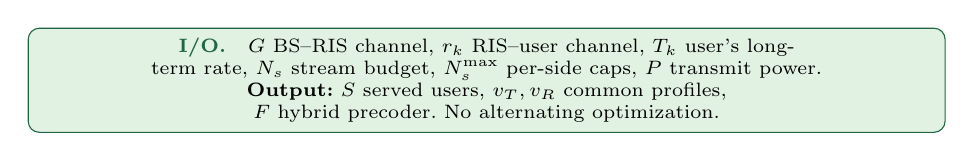
\begin{tikzpicture}
    \node[draw=notegreen, rounded corners, fill=softgreen,
          align=center, inner sep=3.5pt, text width=0.94\textwidth, font=\scriptsize] {
      \textbf{\color{notegreen}I/O.}\quad
      $G$ BS--RIS channel,\
      $r_k$ RIS--user channel,\
      $T_k$ user's long-term rate,\
      $N_s$ stream budget,\
      $N_s^{\max}$ per-side caps,\
      $P$ transmit power.\\
      \textbf{Output:}\
      $S$ served users,\
      $v_T,v_R$ common profiles,\
      $F$ hybrid precoder.\
      No alternating optimization.};
  \end{tikzpicture}
  \vspace{0.25em}
  \begin{center}
  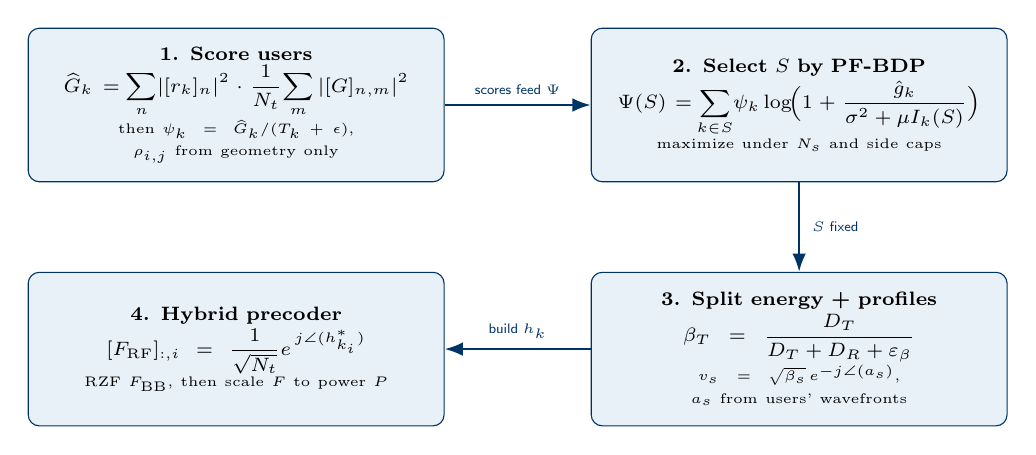
\begin{tikzpicture}[
      arr/.style={-{Latex}, thick, navyblue},
      card/.style={draw=navyblue, rounded corners, fill=softblue,
                   align=center, inner sep=4pt, font=\scriptsize,
                   text width=5.0cm, minimum height=1.95cm},
      lab/.style={font=\tiny\sffamily, text=navyblue, align=center}
    ]
    \node[card] (c1) at (0,1.55) {%
      \textbf{1. Score users}\\[0.1em]
      $\displaystyle\widehat{G}_k=\!\sum_n\!|[r_k]_n|^2\cdot\frac1{N_t}\!\sum_m|[G]_{n,m}|^2$\\
      {\tiny then $\psi_k=\widehat{G}_k/(T_k+\epsilon)$, $\rho_{i,j}$ from geometry only}};
    \node[card] (c2) at (7.15,1.55) {%
      \textbf{2. Select $S$ by PF-BDP}\\[0.1em]
      $\displaystyle\Psi(S)=\!\sum_{k\in S}\!\psi_k\log\!\Bigl(1+\frac{\hat g_k}{\sigma^2+\mu I_k(S)}\Bigr)$\\
      {\tiny maximize under $N_s$ and side caps}};
    \node[card] (c3) at (7.15,-1.55) {%
      \textbf{3. Split energy + profiles}\\[0.1em]
      $\displaystyle\beta_T=\frac{D_T}{D_T+D_R+\varepsilon_\beta}$\\
      {\tiny $v_s=\sqrt{\beta_s}\,e^{-j\angle(a_s)}$, $a_s$ from users' wavefronts}};
    \node[card] (c4) at (0,-1.55) {%
      \textbf{4. Hybrid precoder}\\[0.1em]
      $\displaystyle [F_{\mathrm{RF}}]_{:,i}=\frac1{\sqrt{N_t}}e^{\,j\angle(h_{k_i}^*)}$\\
      {\tiny RZF $F_{\mathrm{BB}}$, then scale $F$ to power $P$}};
    \draw[arr] (c1.east) -- node[lab, above] {scores feed $\Psi$} (c2.west);
    \draw[arr] (c2.south) -- node[lab, right, xshift=1pt] {$S$ fixed} (c3.north);
    \draw[arr] (c3.west) -- node[lab, above] {build $h_k$} (c4.east);
  \end{tikzpicture}
  \end{center}
  \vspace{0.1em}
  {\centering\scriptsize\textit{Per-slot cost $O(N N_t+KN+L_c^2 N_t+2^{L_c}L_c+N_s N)$: only the bitmask term is exponential, in $L_c$ not $N$.}\par}
\end{frame}

%======================================================================
% 6. RESULTS --- Rate
%======================================================================
\begin{frame}{6. Simulation Results (Rate)}
  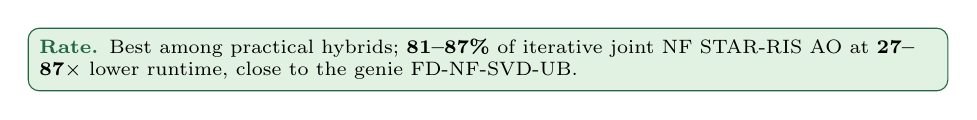
\begin{tikzpicture}
    \node[draw=notegreen, rounded corners, fill=softgreen,
          align=left, inner sep=4pt, text width=0.94\textwidth, font=\scriptsize] {
      \textbf{\color{notegreen}Rate.}
      Best among practical hybrids; \textbf{81--87\%} of iterative joint NF STAR-RIS AO at \textbf{27--87$\times$} lower runtime,
      close to the genie FD-NF-SVD-UB.};
  \end{tikzpicture}
  \vspace{0.2em}
  \begin{columns}[T,onlytextwidth]
    \begin{column}{0.49\textwidth}
      \centering
      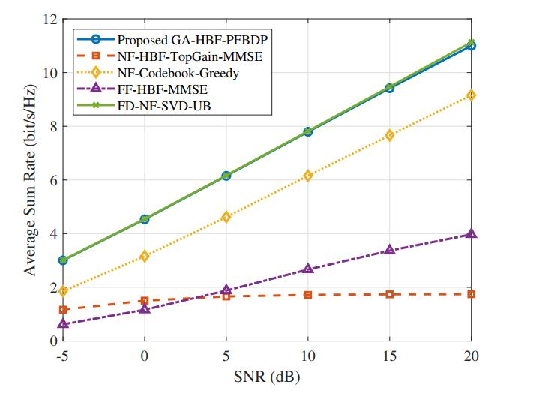
\includegraphics[width=\linewidth,height=0.46\textheight,keepaspectratio]{fig1.pdf}\\[0.1em]
      {\scriptsize Fig.~1. Average sum rate vs.\ SNR (300 drops).}
    \end{column}
    \begin{column}{0.49\textwidth}
      \centering
      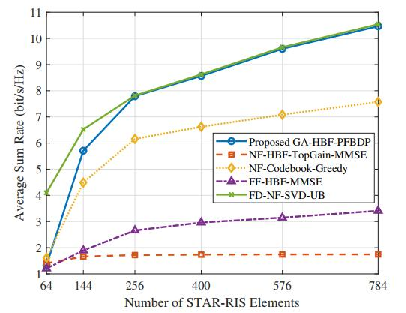
\includegraphics[width=\linewidth,height=0.46\textheight,keepaspectratio]{fig2.pdf}\\[0.1em]
      {\scriptsize Fig.~2. Average sum rate vs.\ STAR-RIS elements (300 drops).}
    \end{column}
  \end{columns}
\end{frame}

%======================================================================
% 7. RESULTS --- Runtime / Users
%======================================================================
\begin{frame}{7. Simulation Results (Runtime and Users)}
  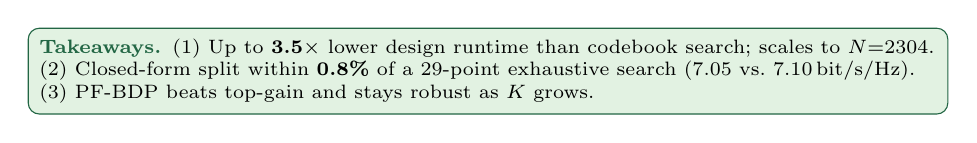
\begin{tikzpicture}
    \node[draw=notegreen, rounded corners, fill=softgreen,
          align=left, inner sep=4pt, text width=0.94\textwidth, font=\scriptsize] {
      \textbf{\color{notegreen}Takeaways.}
      (1)~Up to \textbf{3.5$\times$} lower design runtime than codebook search; scales to $N{=}2304$.
      (2)~Closed-form split within \textbf{0.8\%} of a 29-point exhaustive search (7.05 vs.\ 7.10\,bit/s/Hz).
      (3)~PF-BDP beats top-gain and stays robust as $K$ grows.};
  \end{tikzpicture}
  \vspace{0.2em}
  \begin{columns}[T,onlytextwidth]
    \begin{column}{0.49\textwidth}
      \centering
      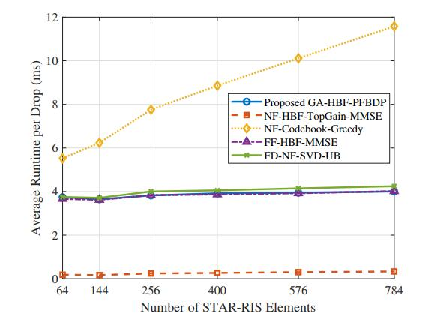
\includegraphics[width=\linewidth,height=0.46\textheight,keepaspectratio]{fig3.pdf}\\[0.1em]
      {\scriptsize Fig.~3. Average design runtime per drop vs.\ STAR-RIS elements.}
    \end{column}
    \begin{column}{0.49\textwidth}
      \centering
      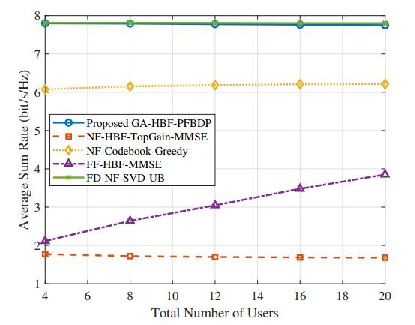
\includegraphics[width=\linewidth,height=0.46\textheight,keepaspectratio]{fig4.pdf}\\[0.1em]
      {\scriptsize Fig.~4. Average sum rate vs.\ total users (300 drops).}
    \end{column}
  \end{columns}
\end{frame}

%======================================================================
% 9. REFERENCES
%======================================================================

\begin{frame}[t]{8. References}
\vspace{-0.4em}

\fontsize{6.5pt}{6.2pt}\selectfont
\begin{thebibliography}{20}
%\setlength{\itemsep}{0.05em}
\setlength{\parsep}{0pt}
\setlength{\parskip}{0pt}

\bibitem{guirado}
M.~A.~ElMossallamy, H.~Zhang, L.~Song, K.~G.~Seddik, Z.~Han, and G.~Y.~Li,
``Reconfigurable intelligent surfaces for wireless communications: Principles, challenges, and opportunities,''
\textit{IEEE Trans.\ Cogn.\ Commun.\ Netw.}, vol.~6, no.~3, pp.~990--1002, 2020.
\bibitem{niu_star}
H.~Niu, Z.~Chu, F.~Zhou, P.~Xiao, and N.~Al-Dhahir,
``Simultaneous transmission and reflection reconfigurable intelligent surface assisted MIMO systems,'' 2021. [Online].
\bibitem{liu_star}
Y.~Liu, J.~Xu, Z.~Wang, X.~Mu, J.~Zhang, and P.~Zhang,
``Simultaneously transmitting and reflecting (STAR) RISs for 6G: Fundamentals, recent advances, and future directions,''
\textit{Frontiers Inf.\ Technol.\ Electron.\ Eng.}, vol.~24, no.~12, pp.~1689--1707, 2023.
\bibitem{hu_lis}
S.~Hu, H.~Wang, and M.~C.~Ilter,
``Design of near-field beamforming for large intelligent surfaces,''
\textit{IEEE Trans.\ Wireless Commun.}, vol.~23, no.~1, pp.~762--774, 2024.
\bibitem{liu_nf_survey}
Y.~Liu, C.~Ouyang, Z.~Wang, J.~Xu, X.~Mu, and A.~L.~Swindlehurst,
``Near-field communications: A comprehensive survey,''
\textit{IEEE Commun.\ Surveys Tuts.}, vol.~27, no.~3, pp.~1687--1728, 2025.
\bibitem{li_star_nf}
H.~Li, Y.~Liu, X.~Mu, Y.~Chen, Z.~Pan, and Y.~C.~Eldar,
``Near-field beamforming for STAR-RIS networks,'' 2023. [Online].
\bibitem{wmmse}
S.~S.~Christensen, R.~Agarwal, E.~de~Carvalho, and J.~M.~Cioffi,
``Weighted sum-rate maximization using weighted MMSE for MIMO-BC beamforming design,''
in \textit{Proc.\ IEEE ICC}, 2009, pp.~1--6.
\bibitem{meng_isac}
C.~Meng, D.~Ma, Z.~Wang, Y.~Liu, Z.~Wei, and Z.~Feng,
``Near-field hybrid beamforming design for modular XL-MIMO ISAC systems,''
\textit{IEEE Trans.\ Commun.}, vol.~73, no.~11, pp.~11840--11854, 2025.
\bibitem{le_bdp}
T.~V.~Le, K.~Lee, and N.~Cong Luong,
``Bitmask dynamic programming for user scheduling in multi-user MIMO mmWave systems,''
\textit{IEEE Commun.\ Lett.}, vol.~27, no.~12, pp.~3365--3369, 2023.
\bibitem{nor_pf}
A.~M.~Nor, O.~Fratu, S.~Halunga, A.~Alyosef, Z.~D.~Zaharis, S.~Rizou, and P.~I.~Lazaridis,
``Demand based proportional fairness scheduling for 5G eMBB services,''
in \textit{Proc.\ IEEE BlackSeaCom}, 2022, pp.~263--268.
\bibitem{nguyen_mmse}
D.~H.~N.~Nguyen, L.~B.~Le, T.~Le-Ngoc, and R.~W.~Heath,
``Hybrid MMSE precoding and combining designs for mmwave multiuser systems,''
\textit{IEEE Access}, vol.~5, pp.~19167--19181, 2017.
%\bibitem{dimic_greedy}
%G.~Dimic and N.~Sidiropoulos,
%``On downlink beamforming with greedy user selection: performance analysis and a simple new algorithm,''
%\textit{IEEE Trans.\ Signal Process.}, vol.~53, no.~10, pp.~3857--3868, 2005.
%\bibitem{song_codebook}
%J.~Song, J.~Choi, and D.~J.~Love,
%``Codebook design for hybrid beamforming in millimeter wave systems,''
%in \textit{Proc.\ IEEE ICC}, 2015, pp.~1298--1303.
\end{thebibliography}
\end{frame}

%======================================================================
% THANK YOU
%======================================================================
\begin{frame}[plain]
\begin{tikzpicture}[remember picture, overlay]
    \fill[navyblue] (current page.south west) rectangle (current page.north east);
\end{tikzpicture}
\vspace{1.5cm}
\begin{center}
    \textcolor{white}{\Huge\textbf{Thank You}}\\[0.8cm]
    \textcolor{white}{\small \confshort}\\[0.45cm]
    
\end{center}
\end{frame}

\end{document}
